\documentclass[12pt]{article}
% \pagestyle{empty}

\setlength{\oddsidemargin}{-0.25 in}
\setlength{\evensidemargin}{-0.25 in}
\setlength{\topmargin}{-0.9 in}
\setlength{\textwidth}{7.0 in}
\setlength{\textheight}{9.0 in}
\setlength{\headsep}{0.75 in}
\setlength{\parindent}{0.3 in}
\setlength{\parskip}{0.1 in}
\usepackage{epsf}
\usepackage{amsmath}
\usepackage{graphicx}
\usepackage{subcaption}
\usepackage{wrapfig}
\def\code#1{\texttt{#1}}

\title{\textbf{Final Project Write-up}}
\author{Tomás Arevalo}
\date{May 3 2023}

\begin{document}
\maketitle

\section{Overview}

\indent The final project tasked me to create my own miniature version of an OCaml interpreter called \\ MiniML. We were given a parser implemented in \code{miniml.ml}, \code{miniml$\textunderscore$lex.mll}, and \code{miniml $\textunderscore$ parse.mly}, as well as some starter code in both \code{expr.ml} and \code{evaulation.ml}. My main responsibility was to create two different interpreters based on either substitution or environment semantic rules. The first was based on substitution semantics which we called \code{eval$\textunderscore$s}; the second was \code{eval$\textunderscore$d}, based on the semantics of a dynamically scoped environment. In order to implement these, I had to implement functions that counted the number of free variables in an expression, functions that took expressions and converted them into strings with either concrete or abstract syntax, and functions that were detailed with all the rules for substitution and for dynamically scoped environment.

After implementing the substitution model and the dynamic model, which can be seen below, it was time to implement my own extensions. Possible extensions varied from adding additional atomic types, modifying the environment semantics to implement a lexical scope, to even adding type inference to the language.

\begin{figure}[h]
  \centering

  \begin{subfigure}{0.45\textwidth}
    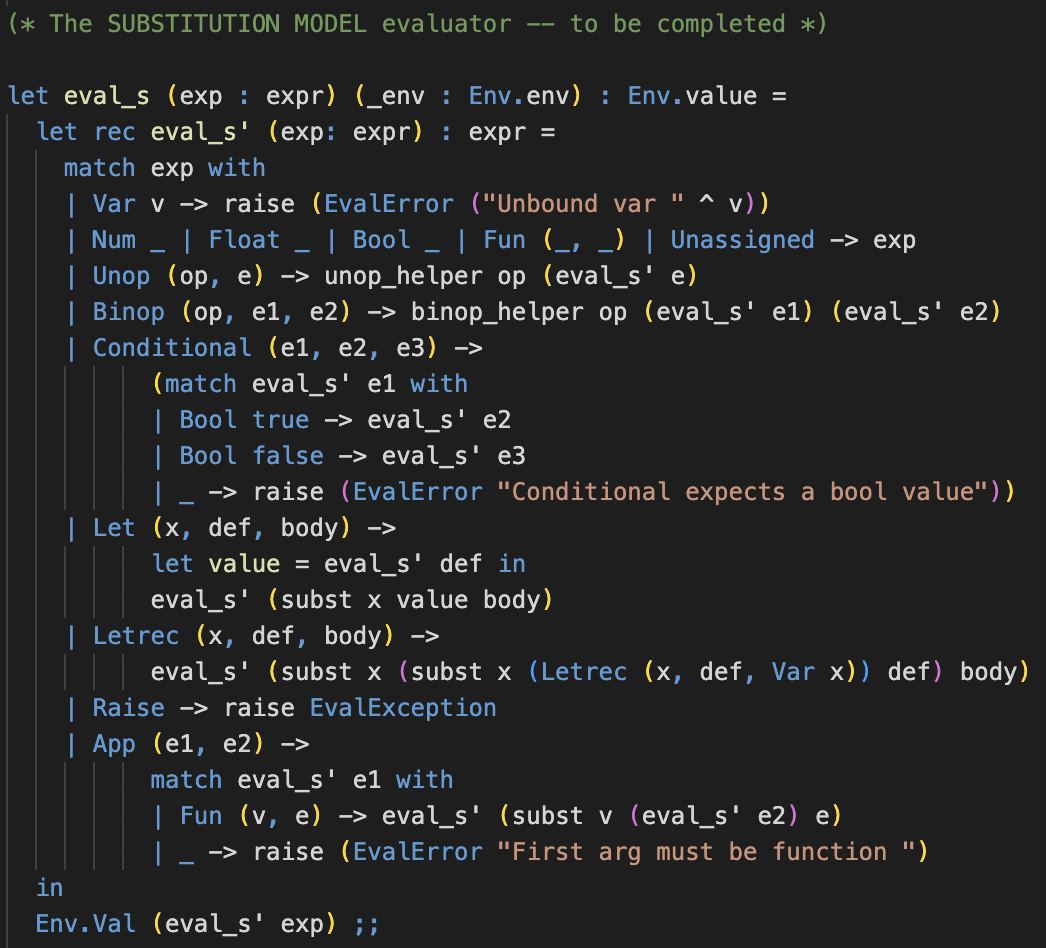
\includegraphics[width=8cm]{Eval_S.png}
  \end{subfigure}
  \hfill
  \begin{subfigure}{0.45\textwidth}
    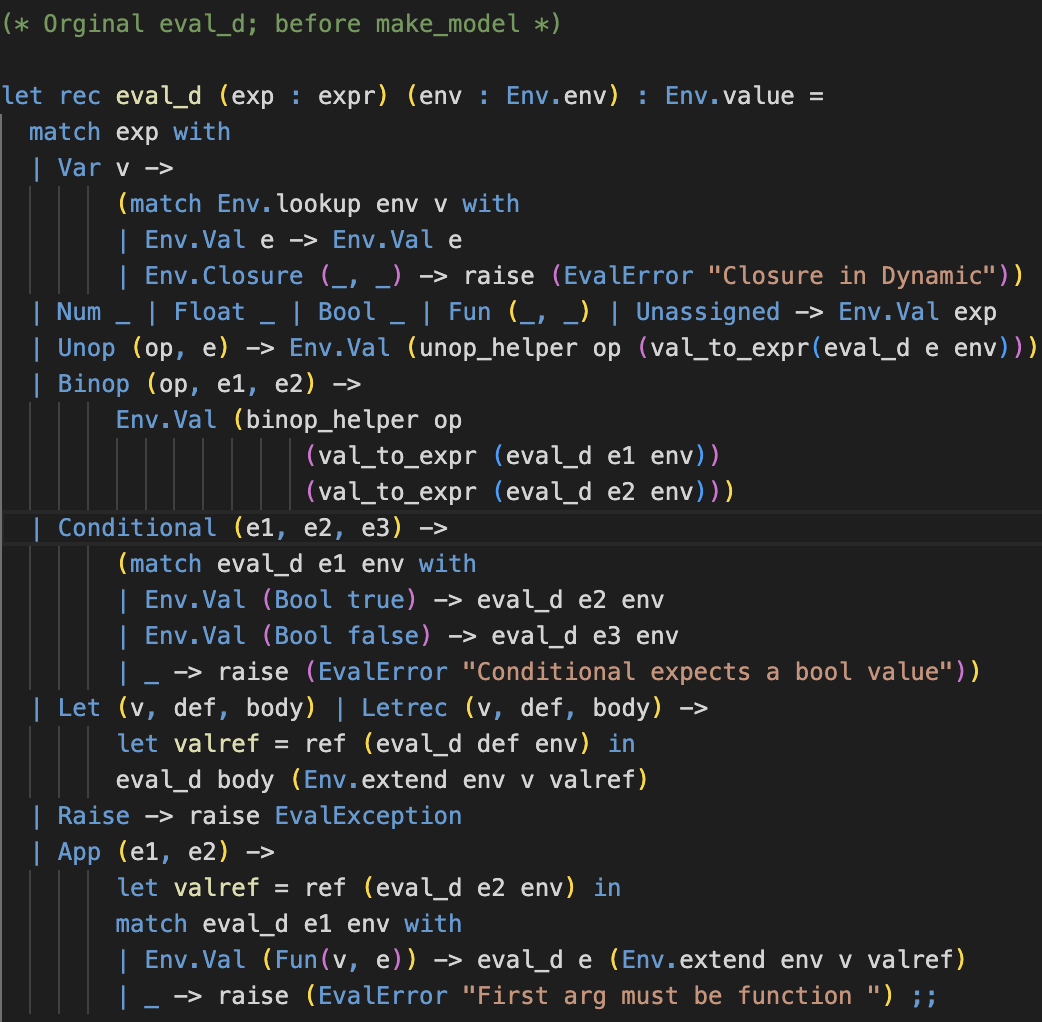
\includegraphics[width=7.5cm]{Eval_D.png}
  \end{subfigure}
\end{figure}

\section{Extensions}
Due to a time constraint and other course work, I implemented a third interpreter based on the environment semantics to manifest a lexical scope, added the atomic type \code{Float} and its corresponding operations, and implemented extra Boolean operations.
\subsection{Lexical Extension}
Ocaml follows the rules of a lexically scoped environment and thus, it was the first extension that I approached. Following the rules in Chapter 19 of the textbook, I quickly realized that a lot of the rules were similar or the same when compared those of \code{eval$\textunderscore$d}. Thus, when implementing \code{eval$\textunderscore$l}, the rules I had to change were that of \code{Fun}, \code{Let} expressions, \code{Letrec} expressions, function \code{App}, and a slight tweak to \code{Var}. This makes sense because the only real differences in ouputs between dynamic and lexical environments, are when storing the values of variables, and then applying them later to functions or Let expressions. We can see this difference below:
\begin{figure}[h]
  \centering
  
  \begin{subfigure}{0.45\textwidth}
    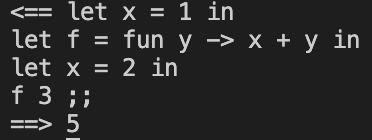
\includegraphics[width=\linewidth]{Dynamic.png}
    \caption{Dynamic Environment Output}
  \end{subfigure}
  \hfill
  \begin{subfigure}{0.45\textwidth}
    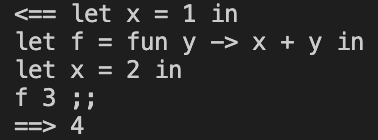
\includegraphics[width=\linewidth]{Lexical.png}
    \caption{Lexical Environment Output}
  \end{subfigure}
\end{figure}

As we can see in the figures above, the dynamic environment doesn't store the original value of $x$, bur rather waits until the function is called, and then uses the most recent value of $x$.  However, in the lexical environment, the function stores the most recent value of $x$ before the function was made, and then preserves it, even if changes to the value of $x$ occur. Below we can see the implemented version of \code{eval$\textunderscore$l}
\begin{center}
    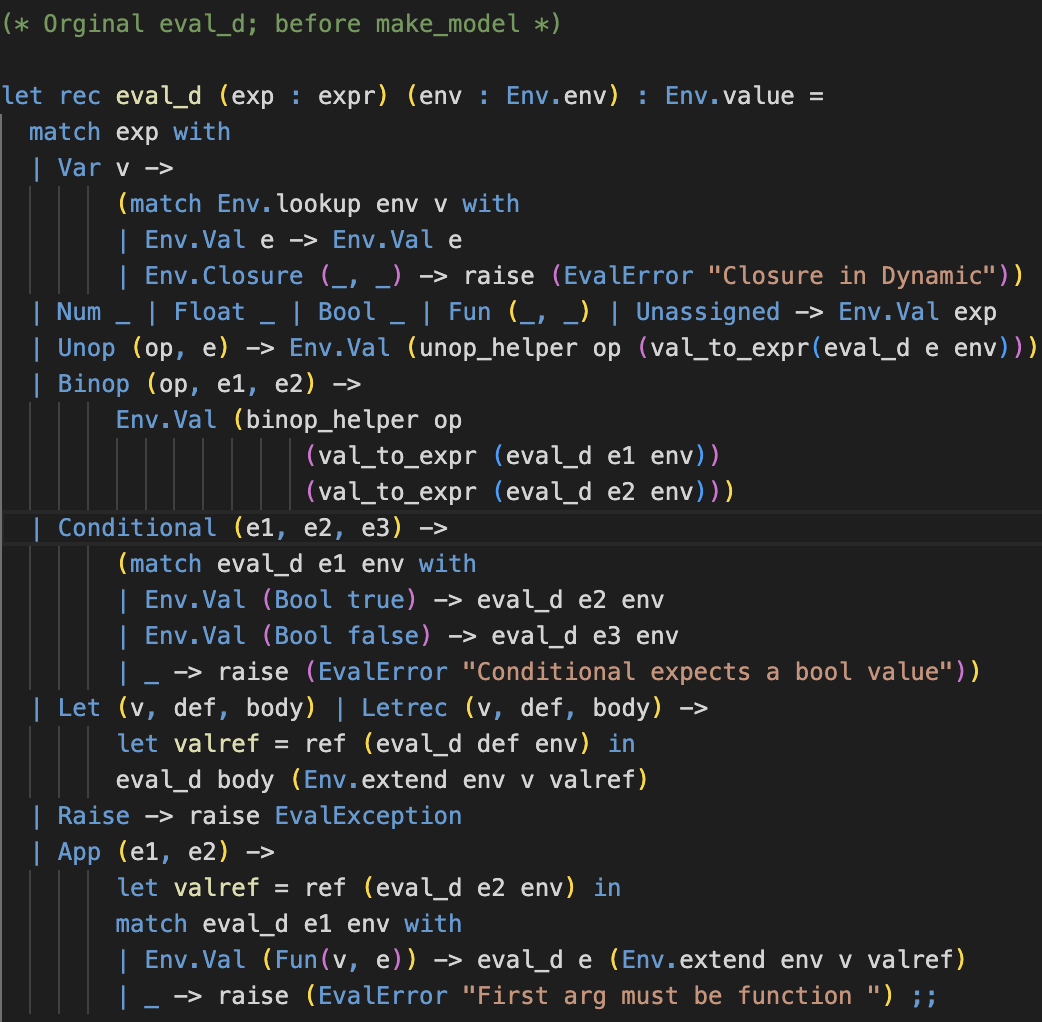
\includegraphics[width=7cm]{Eval_D.png}
\end{center}

\subsection{Float Extension}
The next extension I implemented was adding the \code{Float} atomic type. This was done by adding \code{Float} to the \code{type expr}, and then editing the parser to be be able to identify a \code{Float}. The main edit to the parser, which is shown below, allows the parser to be able to differentiate between a \code{Float} and an \code{Int}.
\begin{center}
    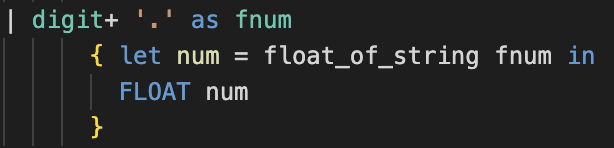
\includegraphics{Float.png}
\end{center}

After doing this, an input such as \code{3.+ 4.} would output \code{7.}, but in Ocaml, this would be an error. Thus, I decided to implement all the operations for a Float which were FloatPlus ($+.$), FloatMinus ($-.$), FloatTimes ($*.$), FloatDivided ($/.$), and FloatNegate ($\sim-.$). (Side note: I also added regular Divided for Num, as it didn't make sense to only have it for floats and not Nums). Adding all these operations were easily added by adding the to the hash table, making them tokens, and then adding their respective grammar rules.
\begin{center}
    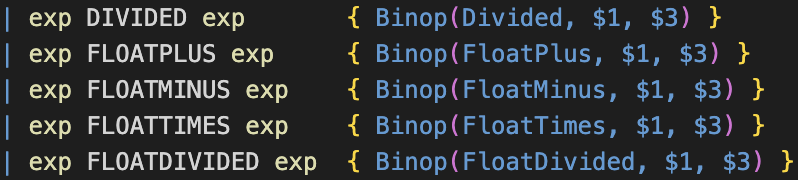
\includegraphics{Float rules.png}
    
\includegraphics{FloatNegate.png}
\end{center}

Obviously, after editing the parser, I went ahead and added all these operations into functions in  \code{expr.ml} and \code{evaluation.ml.}
\subsection{Boolean Extensions}
The last extension I added was Boolean operators such as \code{not, $\&\&$ (AND), || (OR)}. This would allow me to do this like \code{not true = false}, \code{false $\&\&$ true = false}, and \code{false || true = true}. Similar to the \code{Float} operators, it was just adding them to the hash table, making sure `$|$' was in \code{sym []}, making them tokens, and modifying the grammar rules as seen below.
\begin{center}
    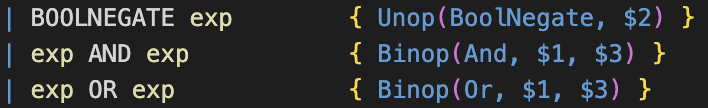
\includegraphics{Bool.png}
\end{center}

\section{Abstraction}
After implementing my extensions, I realized that there was so much redundant code between \code{eval$\textunderscore$d} and \code{eval$\textunderscore$l}. This let me to the idea of making a function \code{make$\textunderscore$model} which would intake the same variables as the dynamic and lexical models, but also intake the type of environment semantic it had to follow (either \code{Dynamic} or \code{Lexical}). Thus, I implemented the following code which saved me 14 lines of codes before adding comments.
\begin{center}
    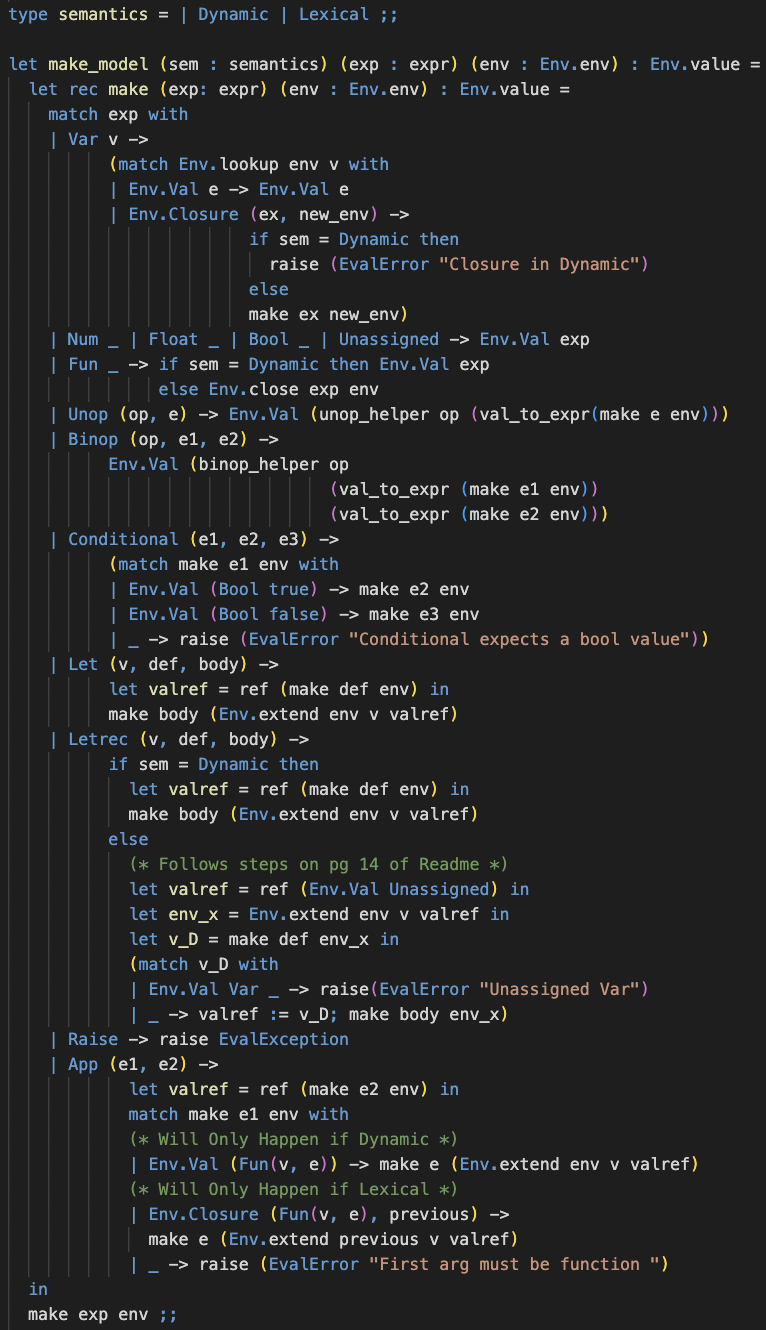
\includegraphics[width=10cm]{makemodel.png}
\end{center}

\end{document}